\section{Recovery Limit under Quality Degradation}
\label{appendix:recovery_limit}

Experiment~03 (\S\ref{sec:eval_catastrophic}) showed that the system
recovers from a silent quality regression (Mistral-Large reward
dropping to $0.75$) within a 608-prompt Phase~3 horizon.  Here we
extend that result across a range of severities.  The system trends
toward recovery at all tested levels---including near-total
degradation---but deeper corruption requires more Phase~3 prompts
under normal conditions to fully converge, and our evaluation horizon
is too short to observe complete recovery at the most extreme levels.
We therefore characterise a finite-horizon recovery envelope: for a
given Phase~3 length, the degradation severity up to which the system
reaches near-Phase~1 performance, and how extending the horizon shifts
that boundary.

\vspace{-0.5ex}
\paragraph{Setup.}
We sweep Mistral-Large's degraded reward from $0.05$ to $0.85$
(normal reward ${\approx}0.92$).  Degradation severity, the x-axis in
Figure~\ref{fig:recovery_limit}a, is the fractional gap between the
degraded reward and the Phase~1 system baseline (${\approx}0.89$),
ranging from ${\approx}4$\% (mild) to ${\approx}94$\% (near-total).
Degradation is modelled as a mean shift: per-prompt rewards are
shifted so the degraded arm's mean equals the target level while
retaining prompt-dependent variation (clipped to $[0,1]$), which is
more realistic than constant-reward replacement.  Cost is held fixed
during Phase~2 so only the reward signal reveals the regression.  All
runs use the moderate budget
($3.3{\times}10^{-4}$--$6.6{\times}10^{-4}$ per prompt), 20~seeds,
and the same hyperparameters as the main experiment.  We define full
recovery as a Phase~3/Phase~1 reward ratio ${\geq}97$\%.

For the extended-horizon evaluation, Phase~3 uses all non-Phase-2
holdout prompts (1{,}216 prompts, $2{\times}$ the base horizon)
without recycling, so the i.i.d.\ arrival assumption is preserved and
extended-horizon results reflect recovery on fresh prompts.

\paragraph{Recovery mechanisms.}
Recovery operates through two mechanisms.  Geometric forgetting
($\gamma{<}1$) exponentially down-weights corrupted Phase-2
observations so that fresh Phase-3 data dominates the mean estimate;
this is the primary driver.  Staleness-driven exploration inflates UCB
variance for non-selected arms and can trigger re-exploration, but
under budget-constrained routing the cost penalty can exceed the
exploration bonus, limiting this effect on its own.  Both mechanisms
act jointly, but the forgetting half-life (${\approx}231$ steps at
$\gamma{=}0.997$) sets the characteristic timescale.

\paragraph{Finite-horizon recovery envelope (Figure~\ref{fig:recovery_limit}a).}
Figure~\ref{fig:recovery_limit}a plots the P3/P1 reward ratio against
degradation severity for two Phase~3 lengths.  At the 608-prompt
horizon (solid blue), full recovery (${\geq}97$\%) is achieved for
degradations up to ${\approx}17$\%, after which the ratio declines
smoothly to a floor of ${\approx}90$\%.  Doubling Phase~3 to 1{,}216
unique prompts (dashed orange) uniformly lifts the curve: the 97\%
boundary shifts to ${\approx}30$\% degradation, and the
severe-degradation floor rises to ${\approx}93$\%.

This uniform lift is consistent with the floor being a finite-horizon
artefact rather than a fundamental limit on recoverable severity:
geometric forgetting continues erasing Phase-2 corruption, so more
Phase-3 prompts yield more recovery.  Within any fixed horizon,
severity beyond ${\approx}50$\% has diminishing marginal impact
because the forgetting dynamics are unchanged; only the initial bias
differs.  At the other extreme, mild degradation (${\leq}10$\%) can
produce P3/P1 ratios above $100$\%: Phase~2 drives the policy away
from the degraded arm, and for some prompts the alternative routing
discovered during degradation is genuinely better than the original
policy.

\begin{figure}[!t]
\centering
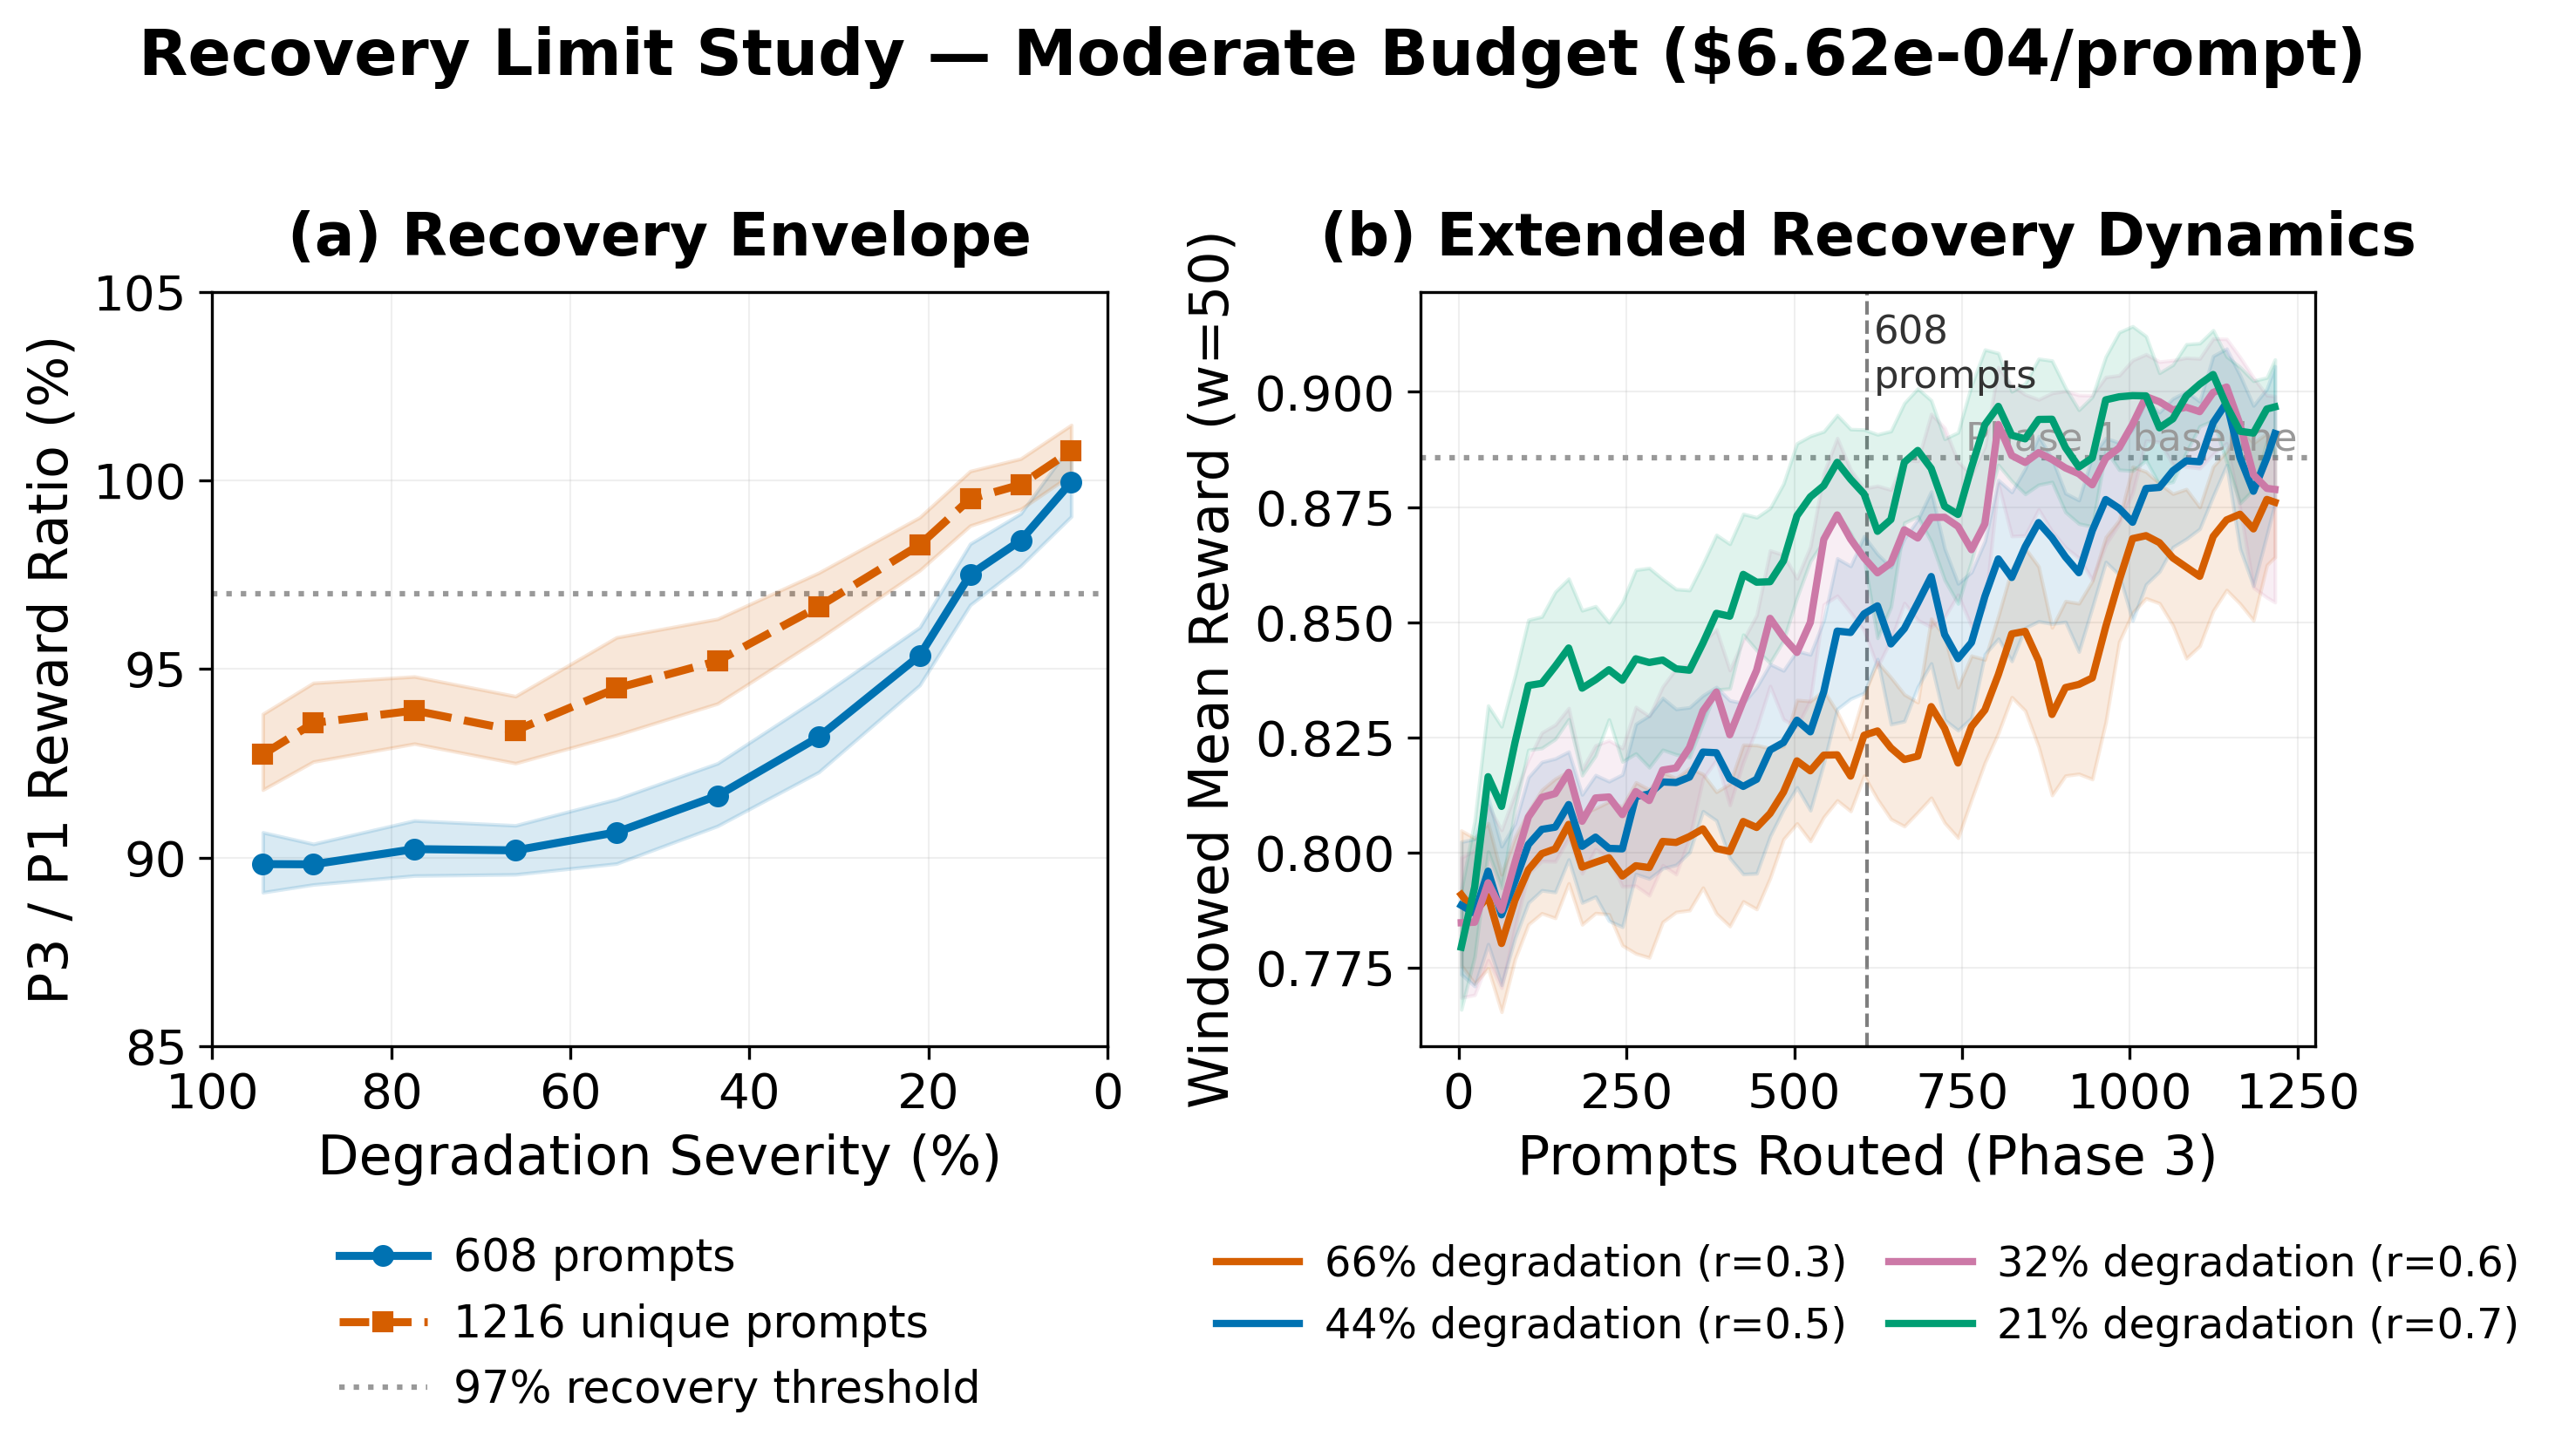
\includegraphics[width=\columnwidth]{../experiments/appendix/recovery_limit/results/recovery_limit.png}
\caption{Recovery limit under quality degradation (moderate budget, \rlNseeds~seeds, 95\% bootstrap CI).
\textbf{(a)}~P3/P1 reward ratio vs.\ degradation severity for \rlPhaseN-prompt (solid) and \rlExtPhaseThreeN-prompt (dashed) Phase~3 horizons.  Dotted line marks the 97\% full-recovery threshold.
\textbf{(b)}~Phase-3 recovery dynamics (50-prompt rolling window) at the extended horizon for four severity levels.  Dotted line marks the Phase~1 baseline; vertical dashed line marks the standard \rlPhaseN-prompt horizon.}
\label{fig:recovery_limit}
\end{figure}

\paragraph{Convergence dynamics (Figure~\ref{fig:recovery_limit}b).}
The extended-horizon time series (50-prompt rolling window) confirm
this interpretation.  All trajectories rise monotonically toward the
Phase~1 baseline with no sign of plateauing, but convergence speed is
severity-dependent: milder degradations reach baseline well before
1{,}216 prompts, while more severe degradations are still improving at
the horizon.  In all cases the confidence bands narrow over time,
indicating stable convergence rather than high-variance oscillation.
The monotonic, non-plateauing trajectories are consistent with
recovery being rate-limited by Phase-3 length rather than
fundamentally bounded by degradation severity, though we cannot
confirm full convergence at the most extreme levels within our
evaluation budget.

\paragraph{Limitations and deployment implications.}
This study evaluates a single budget level and a single-arm,
quality-only degradation; other budgets or simultaneous multi-arm
regressions may behave differently.  For typical silent regressions
(${\leq}20$\%), ParetoBandit recovers automatically within the
608-prompt observation window.  For more severe regressions, recovery
still proceeds but requires a longer Phase~3 horizon; operators can
either allow additional routing time or intervene with an explicit
model demotion to accelerate convergence.
